This tool is based on \unix{}'s \emph{cat}, as it consists in the concatenation of each tune one
after the other in the time perspective. In other words, any voice present in the second tune is
printed after the time offset corresponding to the end of the first tune, and so on.

Some design goals were established:

\begin{enumerate}
  \item The resulting tune's header derives from the first tune which has an actual tune written, in
  other words, at least one \emph{note}.
  \item The \context{} is updated every time a change is detected during the tune's traversal. It is
  a local data structure that comprises the \emph{current voice} and its \emph{key}, \emph{meter},
  \emph{length} and \emph{tempo}. The \emph{number of measures} per voice is recorded separately for
  each tune.
  \item Any \context{} change detected, like the \emph{key} or the \emph{meter}, is written to the
  resulting tune only if it is different from the current \context{}.
  \item For each tune, before appending it to the resulting tune, a verification for missing voices
  is made in the current tune and all prior to that. This way, \measurerests{} can be appended to any
  missing voice in order to ensure that the voice starts at the correct time offset.
  \item In the resulting tune, any voice that has fewer measures than the longest one is appended
  with the necessary \measurerests{} to match the longest.
\end{enumerate}

\subsection*{Algorithm}

\catabc{}'s algorithm is similar to \pasteabc{}'s except that after processing an \abc{} tune with
\dt{}, \measurerests{} may be appended to some voices before and after the actual tune is written.
Since all voices in an \abc{} file are written after the time offset corresponding to the end of the
previous \abc{} file, there may be music missing for some voices from one file to the other, thus
the need for \measurerests{} to fill those "holes".

So the algorithm has the following stages: \textbf{1)} retrieving the header for the resulting tune,
\textbf{2)} printing each tune and any necessary \measurerests{}. In the end, the output generated
is printed to the output.

An algorithmic description is made in algorithm \ref{alg:catabc}.

\begin{enumerate}
  \item The resulting tune's header comes from the first tune with at least one \emph{note} written.

  This stage does exactly the same as \pasteabc{}'s first stage.

  \item For each tune:

  \begin{enumerate}
    \item Applies \dt{} to the current tune;
    \item Appends \measurerests{} to every voice that is present in previous tunes and not in the current one;
    \item Appends \measurerests{} to every voice presented for the first time;
    \item Appends \dt{}'s output, which is the actual tune;
    \item Appends any necessary \measurerests{} to the processed tune (same as stage \textbf{3)} in
    \pasteabc{}'s main algorithm);
  \end{enumerate}

  \begin{program}
    When concatenating tune \emph{A} with tune \emph{B} and tune \emph{B} is being processed, step
    \textbf{b)} appends the \measurerests{} illustrated by the letter \emph{P1} and step \textbf{c)}
    appends the \measurerests{} illustrated by the letter \emph{P2}.

    % \vspace{-1.30cm}
    \begin{center}
      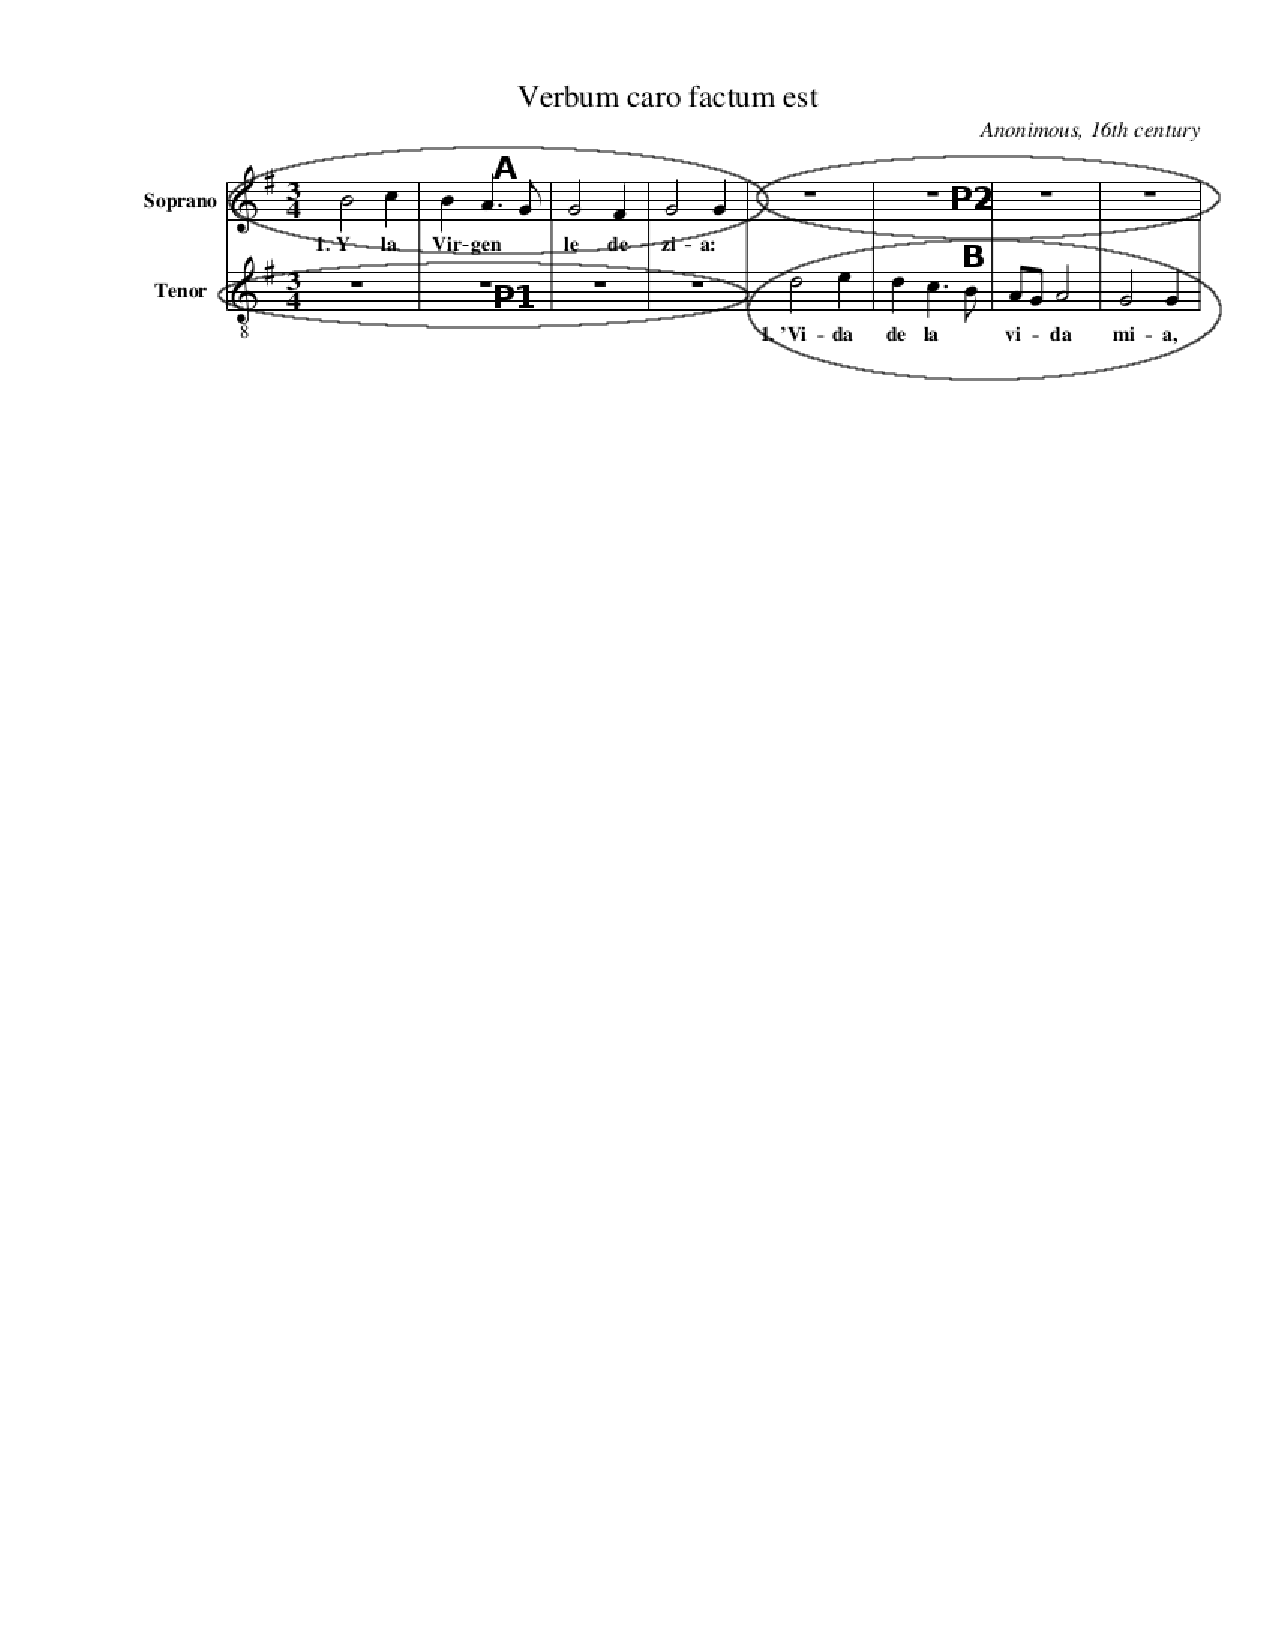
\includegraphics[width=0.8\textwidth, clip=true, trim = 15mm 213mm 0mm 10mm]{img/verbum_measures.pdf}
    \end{center}

    \caption{Appending necessary \measurerests{}}
  \end{program}

  Each individual result is concatenated into the resulting tune.\\

  The set of \abcdtrules{} used in this stage is the same as in \pasteabc{}'s second stage. However,
  \catabc{} provides two more options for concatenating tunes: inserting a number of \measurerests{}
  at the beginning of each tune (option \emph{-d}) and repeating each tune a number of times (option
  \emph{-r}).

  To implement the first option, some modifications were made to the set of \abcdtrules{}:

  \begin{itemize}
    \item The default transformation for each \abcelement{} is not \toabc{}, but instead a local
    function that, once for each voice, inserts a \measurerest{} with the request length before the
    element itself and also updates the \context{}'s measure count for that voice.
    \item The \context{}'s measure count update is made when a \emph{bar} or a \emph{mrest} is
    found.
  \end{itemize}

  Those modifications are described in table \ref{tab:cat_snd_stg_rules}.

  \begin{center}
    \begin{table}[h]
      \begin{tabular}{|p{2.5cm}|p{4.75cm}|p{8cm}|}
        \hline
        Actuator & Transformation (Perl) & Notes\\
        \hline
        \hline
        \emph{bar} & update\_measure\_count(1); insert\_canon\_delta(); &
        \emph{update\_measure\_count} is a local function that increments, in this case by 1, the
        \context{}'s measure count for the current voice. \emph{insert\_canon\_delta} is a local
        function that inserts a \measurerest{} before the element itself, once for each voice.
        \\
        \hline

        \hline
        \emph{mrest} & update\_measure\_count( \$sym->\{info\}->\{len\} - 1 );
        insert\_canon\_delta(); &
        \emph{\$sym} is the \abcelement{} currently being processed, a \measurerest{}.
        \emph{\$sym->\{info\}->\{len\}} is the number of measures in rest.
        \\
        \hline

        \hline
        \emph{-default} & insert\_canon\_delta(); &
        \\
        \hline
      \end{tabular}
      \caption{\abcdtrules{} for \catabc{}'s second stage}
      \label{tab:cat_snd_stg_rules}
    \end{table}
  \end{center}

  The second option is obtained by simply repeating steps \textbf{a} to \textbf{e} a requested
  number of times.
\end{enumerate}

\begin{algorithm}[h]
  \KwIn{abc\_tunes}
  \ForAll{$ tune \in abc\_tunes $}{
    $header \gets dt(tune,$ rules from table \ref{tab:paste_fst_stg_rules}$)$ \hfill //1)\\
  }
  \ForAll{$ tune \in abc\_tunes $}{
    \For{$ 0 .. $ value of \emph{-r} option }{
      $c\_tune \gets dt(tune,$ rules from tables \ref{tab:paste_snd_stg_rules} and \ref{tab:cat_snd_stg_rules}$)$ \hfill //2-a)\\
      $res \gets res$ ++ $add\_measures\_to\_missing\_voices()$ \hfill //2-b)\\
      $res \gets res$ ++ $add\_measures\_to\_new\_voices()$ \hfill //2-c)\\
      $res \gets res$ ++ $c\_tune$ \hfill //2-d)\\
      $res \gets res$ ++ $add\_measures()$ \hfill //2-e)\\
    }
  }
  \Return{$header$ ++ $res$}
  \caption{\catabc{}'s algorithm}
  \label{alg:catabc}
\end{algorithm}

\subsection*{Usage}

Listing \ref{lst:catabcman} shows \catabc{}'s manual.\\

\lstinputlisting[caption={\catabc{}'s manual},label={lst:catabcman},captionpos=t,abovecaptionskip=-\medskipamount]{misc/cat_manual.tex}

Listing \ref{lst:cat_abc_by_example} shows a usage example for \catabc{}. It reads tunes
\textbf{201.abc} (listing \ref{lst:verbum_s2_p1}) and \textbf{303.abc} (listing
\ref{lst:verbum_s3_p3}) and the output is shown in listing \ref{lst:verbum_s2_p1_s3_p3_cated} with
its respective score (figure \ref{fig:verbum_s2_p1_s3_p3}).\\

\begin{lstlisting}[caption={\catabc{} by example},label={lst:cat_abc_by_example},captionpos=t,abovecaptionskip=-\medskipamount]
cat_abc 201.abc 303.abc
\end{lstlisting}

\lstinputlisting[caption={Verbum caro factum est: Section 2; Part 1 - Soprano},label={lst:verbum_s2_p1},captionpos=t,abovecaptionskip=-\medskipamount]{misc/201.tex}

\vspace{-1.30cm}
\begin{figure}[h]
  \begin{center}
    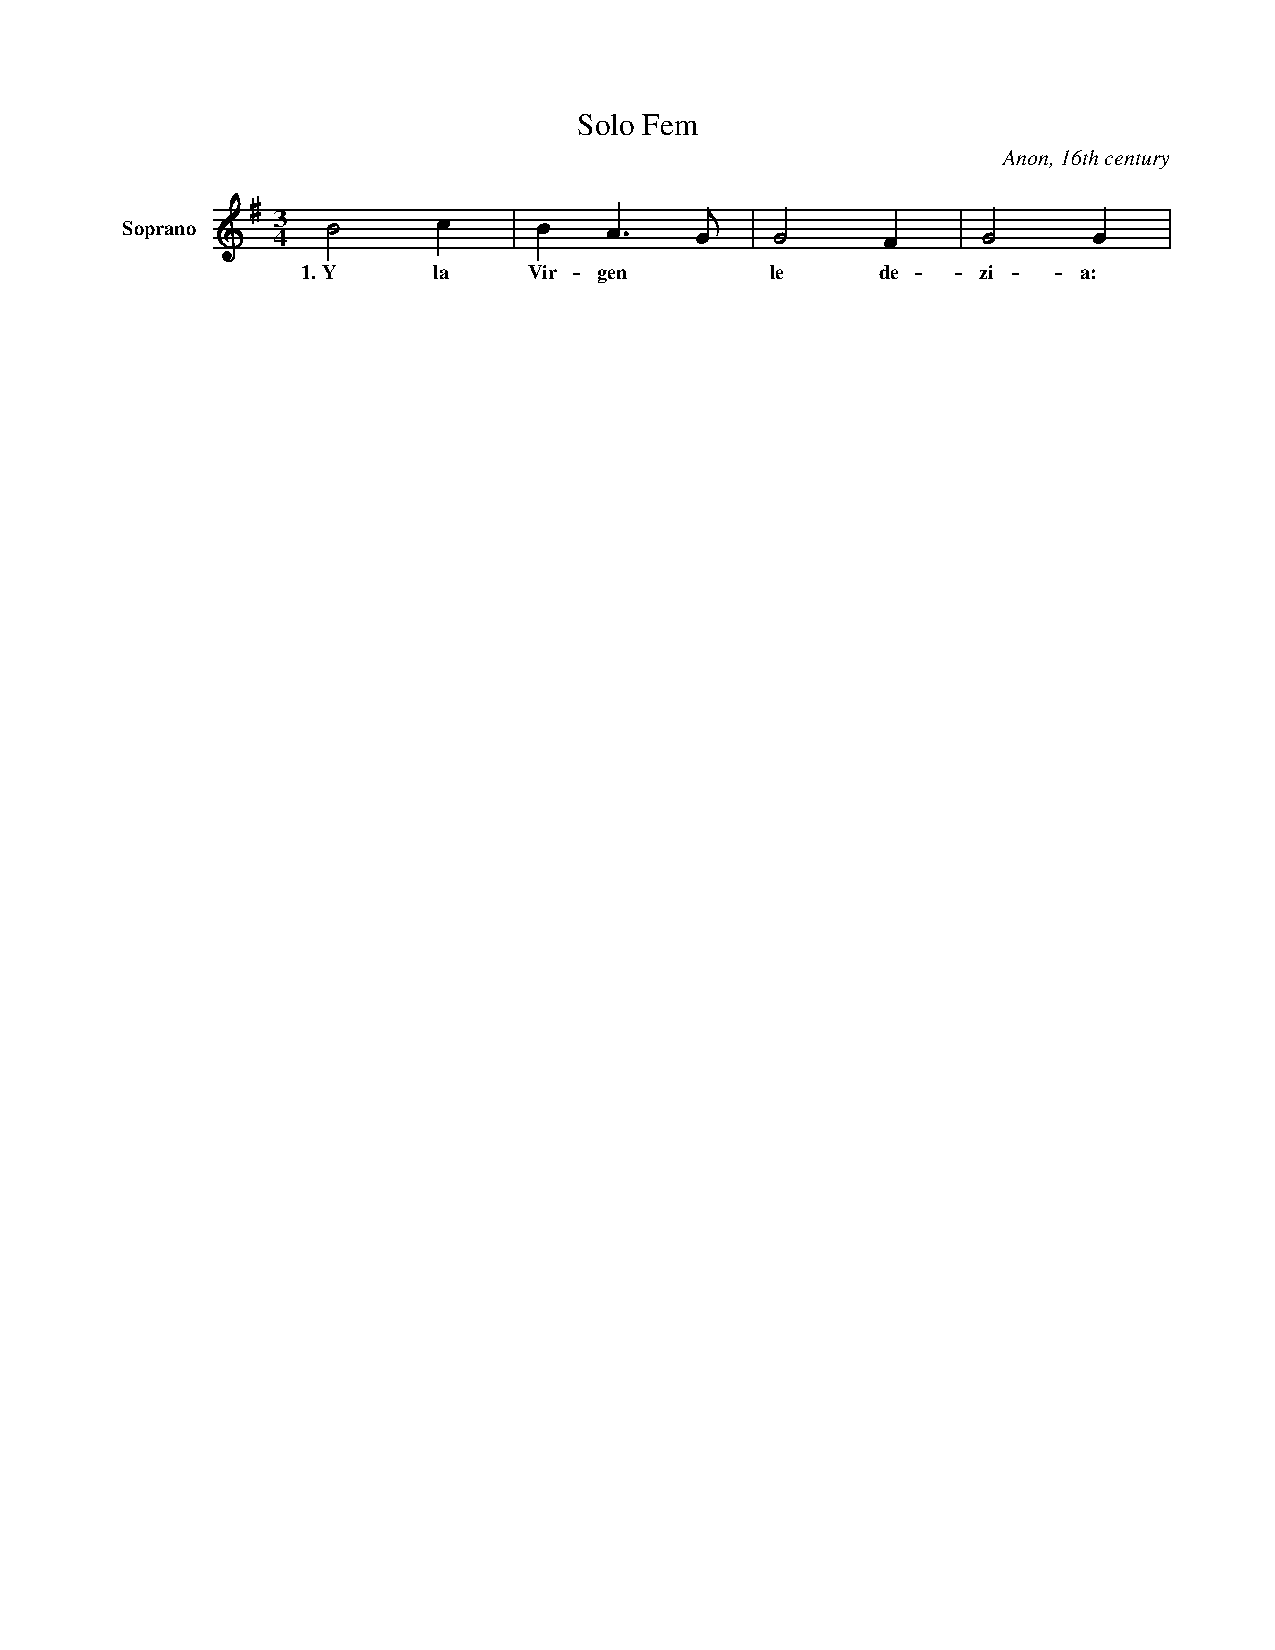
\includegraphics[width=0.8\textwidth, clip=true, trim = 15mm 231mm 0mm 0mm]{img/201.pdf}
    \caption{Verbum caro factum est: Section 2; Part 1 - Soprano (Score)}
  \end{center}
\end{figure}

\lstinputlisting[caption={Verbum caro factum est: Section 3; Part 3 - Tenor},label={lst:verbum_s3_p3},captionpos=t,abovecaptionskip=-\medskipamount]{misc/303.tex}

% \vspace{-1.30cm}
\begin{figure}[H]
  \begin{center}
    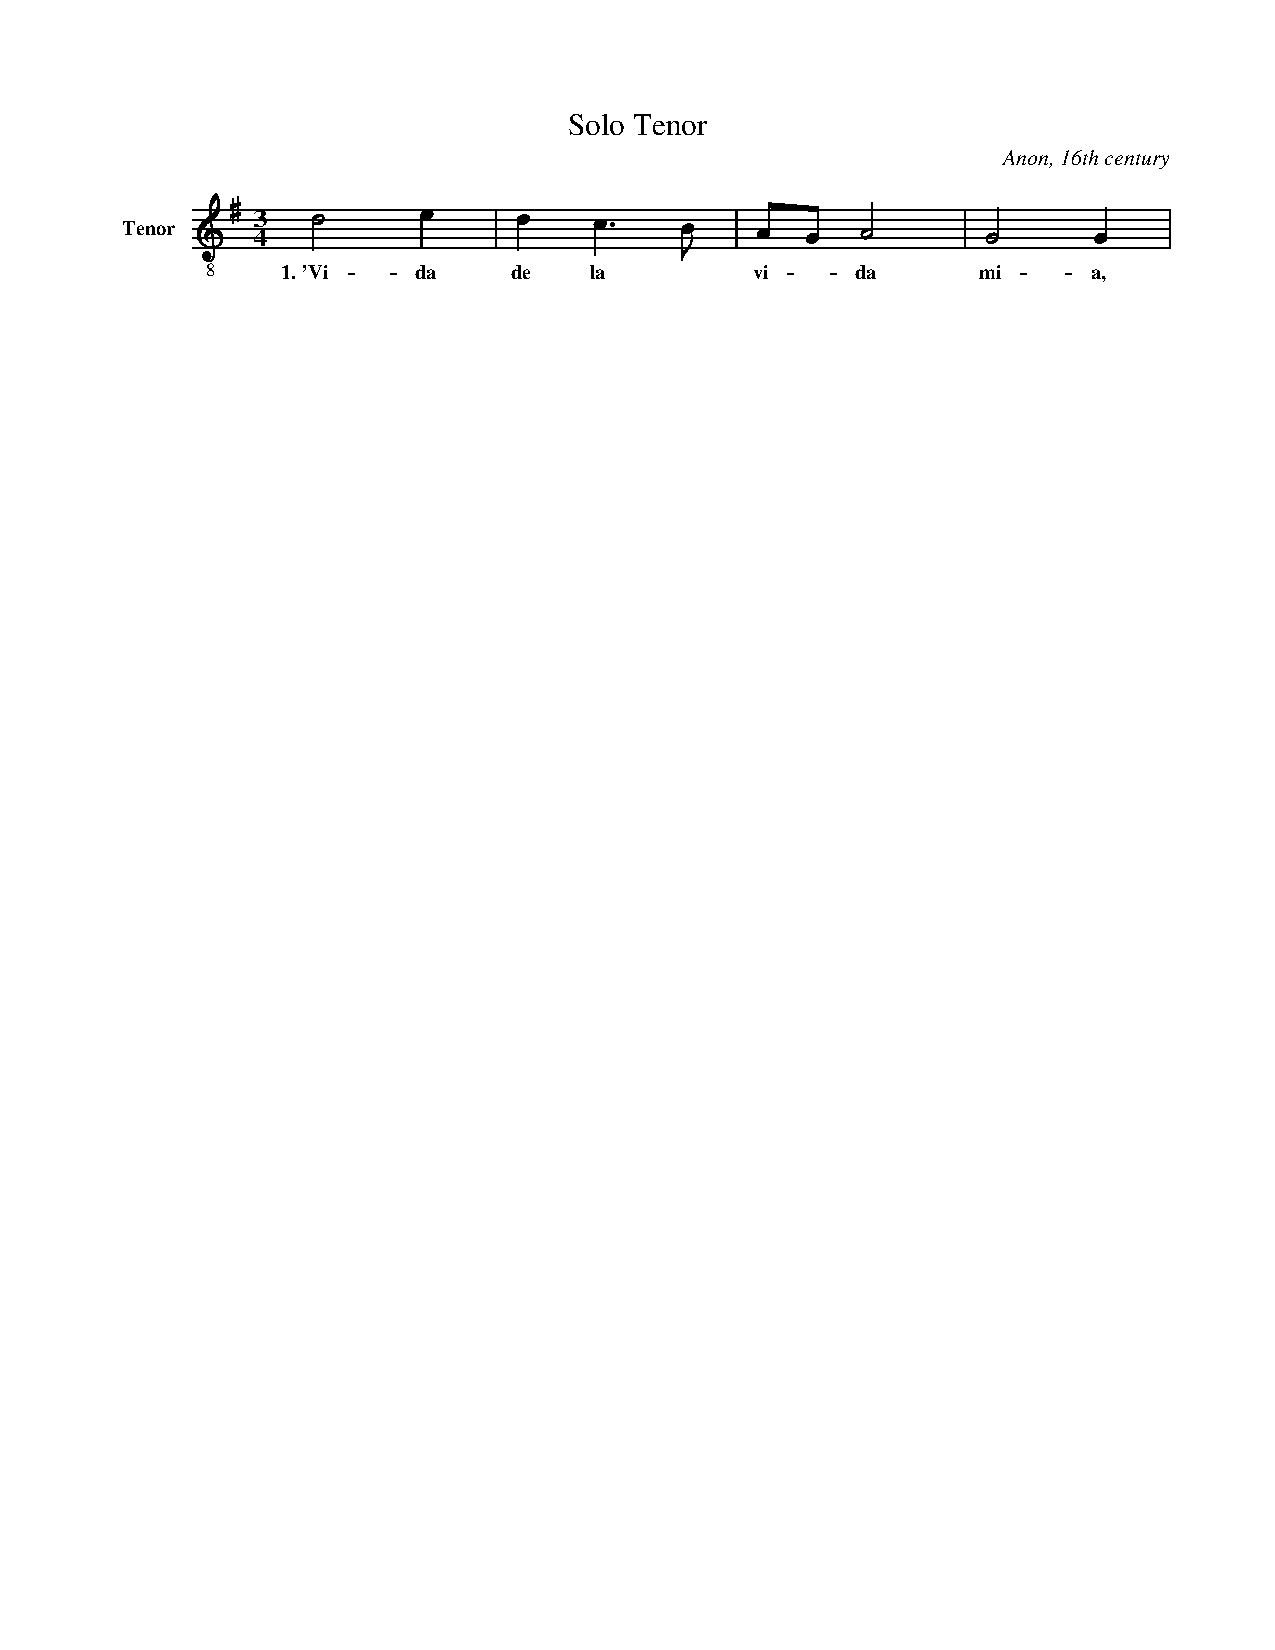
\includegraphics[width=0.8\textwidth, clip=true, trim = 15mm 231mm 0mm 0mm]{img/303.pdf}
    \caption{Verbum caro factum est: Section 3; Part 3 - Tenor (Score)}
  \end{center}
\end{figure}

\lstinputlisting[caption={Verbum caro factum est: Section 2; Part 1 \& Section 3: Part 3},label={lst:verbum_s2_p1_s3_p3_cated},captionpos=t,abovecaptionskip=-\medskipamount]{misc/verbum_s2_p1_s3_p3_cated.tex}

\vspace{-1.50cm}
\begin{figure}[H]
  \begin{center}
    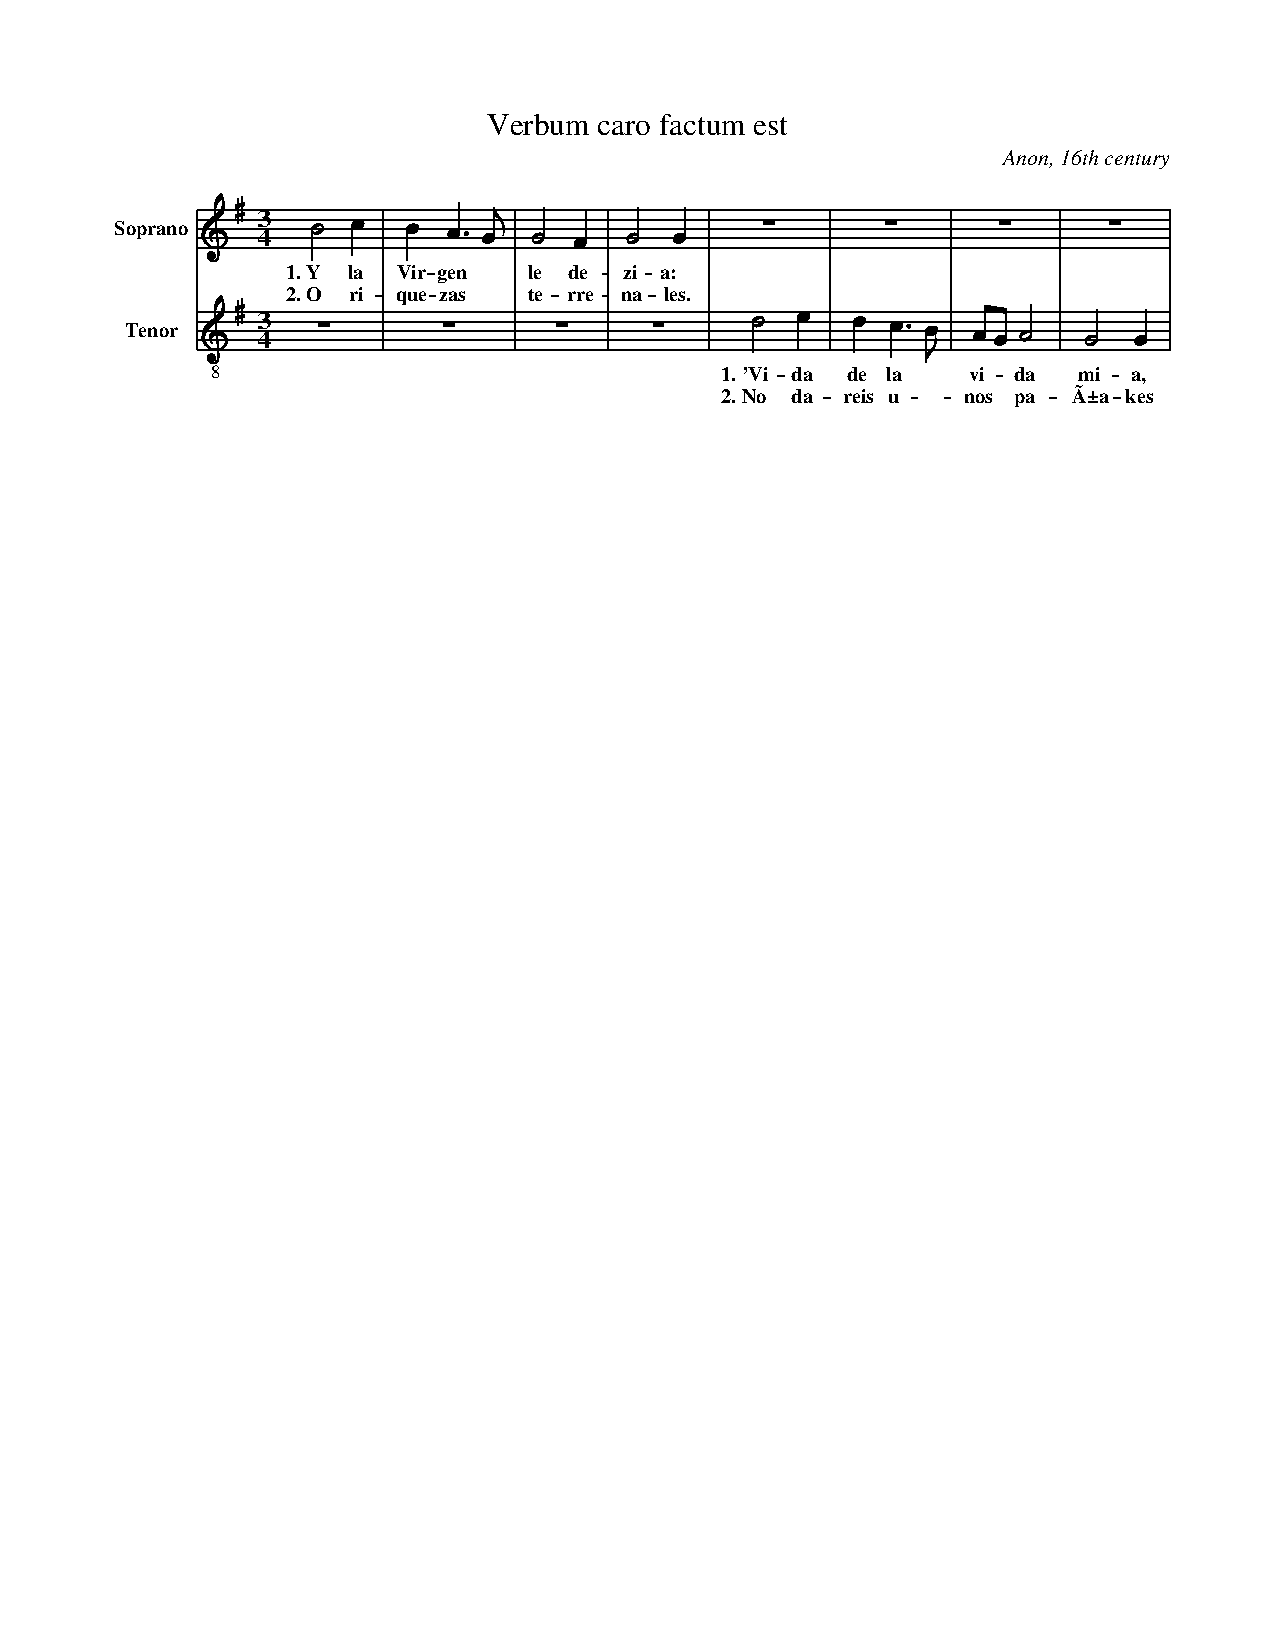
\includegraphics[width=0.8\textwidth, clip=true, trim = 18mm 210mm 16mm 0mm]{img/verbum_s2_p1_s3_p3.pdf}
    \caption{Verbum caro factum est: Section 2; Part 1 \& Section 3: Part 3 (Score)}
    \label{fig:verbum_s2_p1_s3_p3}
  \end{center}
\end{figure}
